\documentclass[conference]{IEEEtran}
\usepackage{cite}
\usepackage{amsmath,amssymb}
\usepackage{graphicx}
\usepackage{booktabs}
\usepackage{xcolor}
\usepackage{algorithm}
\usepackage{algpseudocode}
\newcommand{\todo}[1]{\textcolor{red}{[TODO: #1]}}

\begin{document}

\title{Harmonic-Percussive Source Separation of Music Signals Using STFT and Median Filtering: Mask, Filter-Length, and Window-Size Analysis}

\author{\IEEEauthorblockN{Mohammed Ayaan Azmath, Dr. Bhasker Dappuri}
\IEEEauthorblockA{Chaitanya Bharathi Institute of Technology\\
Hyderabad, India}}

\maketitle

\begin{abstract}
Harmonic-percussive source separation (HPSS) splits a music signal into sustained tonal sounds and short transient sounds, and is a common preprocessing step in music analysis and audio editing. This paper studies median-filtering HPSS in the short-time Fourier transform (STFT) domain. The method computes a magnitude spectrogram, applies median filters along the time and frequency axes to enhance harmonic and percussive structures, builds binary or soft time-frequency masks from the two enhanced spectrograms, and reconstructs both components with the inverse STFT. The study examines how mask type, median-filter length, window length, and additive noise affect separation. On a 10~s real music excerpt sampled at 44.1~kHz, soft-mask HPSS assigned 89.2\% of the signal energy to the harmonic component and 1.5\% to the percussive component, and the two components reconstructed the input with a normalized error of about $10^{-16}$. A controlled synthetic benchmark with known reference components is used to quantify separation by signal-to-distortion ratio (SDR). Relative to using the mixture as the estimate, the default soft-mask method raised the percussive SDR from $-13.1$~dB to 1.9~dB, binary masks reached 21.2~dB and 8.1~dB for the harmonic and percussive components, and SDR increased with both median-filter length and window length over the tested ranges. The study uses one real clip and a simple synthetic benchmark, and it does not compare against learned separation methods, so the results describe the behavior of the classical method rather than a new state of the art.
\end{abstract}

\begin{IEEEkeywords}
harmonic-percussive source separation, STFT, median filtering, spectrogram, time-frequency masking, audio signal processing
\end{IEEEkeywords}

\section{Introduction}
Music signals are typically a mixture of sustained tonal sounds, such as vocals, strings, and keyboards, and short transient sounds, such as drum hits. Separating the two is useful for music analysis tasks such as chord and rhythm analysis, and for audio editing and remixing \cite{muller2015}. In a spectrogram the two classes have clear geometry. Sustained tonal sounds appear as horizontal ridges because their energy persists in time at nearly fixed frequencies, whereas transient sounds appear as vertical ridges because their energy is short in time and spread over many frequencies.

Several approaches exploit this structure. Independent subspace analysis has been used to extract drum tracks from polyphonic music \cite{uhle2003}. Ono et al.\ formulated HPSS as an optimization on the spectrogram using complementary diffusion \cite{ono2008}. Fitzgerald proposed median filtering of the spectrogram along the time and frequency axes as a simple alternative, with both binary and soft (Wiener-like) masks \cite{fitzgerald2010}. Tachibana et al.\ used the anisotropic smoothness of spectrograms \cite{tachibana2014}, and Driedger et al.\ extended median-filter HPSS with a third, residual component for sounds that are neither clearly harmonic nor percussive \cite{driedger2014}.

This paper considers a narrower question: how do the practical design choices of the median-filtering method, namely the mask type, the median-filter length, the STFT window length, and additive noise, affect its separation quality, and how well can the result be judged when reference stems are unavailable? The contributions are:
\begin{enumerate}
\item a complete MATLAB implementation of median-filter HPSS with binary and soft masks and an edge-safe STFT reconstruction;
\item an evaluation on a real music excerpt using spectrograms, masks, waveforms, energy distribution, and reconstruction error;
\item a controlled synthetic benchmark with known harmonic and percussive references, used to measure SDR as a function of mask type, filter length, window length, and noise level; and
\item an explicit statement of what these measurements can and cannot show.
\end{enumerate}
The paper treats the results as a study of a classical method. It does not claim an improvement over published HPSS methods.

\section{Signal Model and Spectrogram Structure}
\subsection{Additive Harmonic-Percussive Model}
The observed signal is modeled as
\begin{equation}
x[n]=x_H[n]+x_P[n],
\end{equation}
where $x_H[n]$ is the harmonic component, a sum of sinusoids with slowly varying amplitude and frequency, and $x_P[n]$ is the percussive component, made of short broadband bursts. The goal is to estimate $x_H[n]$ and $x_P[n]$ from $x[n]$ alone.

\subsection{Short-Time Fourier Transform}
The STFT of $x[n]$ is \cite{allen1977}
\begin{equation}
X(m,k)=\sum_{n=0}^{N-1} x[n+mH]\,w[n]\,e^{-j2\pi kn/N},
\end{equation}
where $w[n]$ is the analysis window, $N$ is the frame length, $H$ is the hop size, $m$ is the frame index, and $k$ is the frequency bin. The magnitude spectrogram is $S(m,k)=|X(m,k)|$. A tonal component produces a ridge along $m$ at a fixed $k$, and an impulsive component produces a ridge along $k$ at a fixed $m$ \cite{oppenheim}.

\section{HPSS Method}
\subsection{Median Filtering}
Harmonic- and percussive-enhanced spectrograms are obtained by median filtering $S$ along each axis:
\begin{align}
\mathcal{H}(m,k) &= \operatorname{median}\{S(m-\ell_h,k),\dots,S(m+\ell_h,k)\},\\
\mathcal{P}(m,k) &= \operatorname{median}\{S(m,k-\ell_p),\dots,S(m,k+\ell_p)\},
\end{align}
where $L_h=2\ell_h+1$ and $L_p=2\ell_p+1$ are the filter lengths. Filtering along time removes short vertical events and keeps horizontal ridges. Filtering along frequency removes narrow tonal peaks and keeps vertical ridges. Near the signal and spectrum edges the window is shortened.

\subsection{Mask Construction}
The binary masks are
\begin{equation}
M_H(m,k)=\begin{cases}1,&\mathcal{H}(m,k)\ge\mathcal{P}(m,k)\\0,&\text{otherwise}\end{cases},\quad M_P=1-M_H.
\end{equation}
The soft masks are
\begin{equation}
M_H=\frac{\mathcal{H}^{2}}{\mathcal{H}^{2}+\mathcal{P}^{2}+\epsilon},\qquad M_P=\frac{\mathcal{P}^{2}}{\mathcal{H}^{2}+\mathcal{P}^{2}+\epsilon},
\end{equation}
where $\epsilon$ is a small constant that avoids division by zero. Soft masks sum to one at every time-frequency point, so no energy is discarded at the mask stage.

\subsection{Reconstruction}
The masks are applied to the complex STFT, $X_H=M_H\odot X$ and $X_P=M_P\odot X$, and the inverse STFT with overlap-add \cite{griffin1984} gives $x_H[n]$ and $x_P[n]$. The inverse transform divides by the accumulated window overlap, which is close to zero at the first and last samples of a Hann window. Without precaution this produces large spikes at both ends of the output. The implementation therefore zero-pads the input before the STFT and removes the padding after reconstruction (Algorithm~\ref{alg:hpss}).

\begin{algorithm}[t]
\caption{Median-filter HPSS}
\label{alg:hpss}
\begin{algorithmic}[1]
\Require signal $x[n]$, $N$, $H$, $L_h$, $L_p$, mask type
\State $x_{\text{pad}}\gets[\mathbf{0}_N,\;x,\;\mathbf{0}_{2N}]$
\State $X\gets\text{STFT}(x_{\text{pad}})$, $S\gets|X|$
\State $\mathcal{H}\gets$ median filter of $S$ along time, length $L_h$
\State $\mathcal{P}\gets$ median filter of $S$ along frequency, length $L_p$
\State Compute $M_H$, $M_P$ (binary or soft)
\State $X_H\gets M_H\odot X$, $X_P\gets M_P\odot X$
\State $x_H,x_P\gets\text{ISTFT}(X_H),\text{ISTFT}(X_P)$
\State Remove the first $N$ samples and trim to $\text{length}(x)$
\State \Return $x_H,\,x_P$
\end{algorithmic}
\end{algorithm}

\section{Experimental Methodology}
\subsection{Real Music Excerpt}
The real test signal is a 10~s mono excerpt of the piece ``Solitude Waltz'' (sad piano music) by Brukowskij, obtained from uppbeat.io, sampled at 44.1~kHz and normalized to unit peak amplitude. The system is implemented in MATLAB R2026b using the Signal Processing Toolbox functions \texttt{stft} and \texttt{istft}, and median filtering is performed with \texttt{movmedian}. No reference harmonic or percussive stems are available for this excerpt.

\subsection{Synthetic Benchmark}
To obtain ground truth, a 10~s synthetic signal is generated at 22.05~kHz. The harmonic part consists of four chords of 2.5~s each, where every note has five harmonics with amplitudes decreasing as $1/h$ and a slowly decaying envelope. The percussive part is a drum-like pattern on a 0.25~s grid made of a decaying low-frequency sinusoid (kick), a decaying noise burst (snare), and a short high-pass noise burst (hi-hat). Both parts are scaled by a common factor so that the mixture has unit peak amplitude, and the random seed is fixed at 2026. In this benchmark the harmonic component carries about 20 times the energy of the percussive component (13.1~dB).

\subsection{Parameters and Sweeps}
Table~\ref{tab:params} lists the default parameters. The sweeps are $L_h=L_p\in\{5,9,17,31,51\}$ bins, $N\in\{512,1024,2048\}$ with $H=N/4$, mask type in \{binary, soft\}, and mixture SNR in $\{\infty,20,10,0\}$~dB for added white Gaussian noise.

\begin{table}[t]
\centering
\caption{Default parameters}
\label{tab:params}
\begin{tabular}{ll}
\toprule
Parameter & Value\\
\midrule
Sampling rate (real clip) & 44100 Hz\\
Sampling rate (synthetic) & 22050 Hz\\
Window & Hann, 1024 samples\\
Hop size & 256 samples\\
Time-median length $L_h$ & 17\\
Frequency-median length $L_p$ & 17\\
Mask (default) & soft\\
\bottomrule
\end{tabular}
\end{table}

\subsection{Performance Measures}
Three measures are used. The energy share of each component is $E_H/E_x$ and $E_P/E_x$ with $E_x=\sum_n x^2[n]$. The normalized reconstruction error is $\|x-(x_H+x_P)\|^2/\|x\|^2$. For the synthetic benchmark, where references $x_H^{\text{ref}}$ and $x_P^{\text{ref}}$ are known, the signal-to-distortion ratio of an estimate $\hat{s}$ of a reference $s$ is
\begin{equation}
\text{SDR}=10\log_{10}\frac{\|s\|^2}{\|s-\hat{s}\|^2}.
\end{equation}
This is the simple form of SDR and is not the full BSS Eval decomposition, which allows a filtered version of the reference \cite{vincent2006}. As a baseline, the SDR obtained by using the unseparated mixture as the estimate of each component is also reported. When noise is added, the references remain the clean components, so the noise counts as distortion.

\section{Results}
\subsection{Real Music Excerpt}
Using soft masks, the harmonic component contains 89.2\% of the original signal energy and the percussive component 1.5\%. The two do not sum to 100\% because energy is not additive when the components overlap, but the normalized reconstruction error is about $10^{-16}$, so $x_H+x_P$ recovers the original signal to numerical precision. The low percussive share indicates that the excerpt is dominated by sustained tonal content.

Fig.~\ref{fig:spec} shows the original spectrogram and the two separated components. The harmonic component retains the horizontal ridges at low frequencies, below roughly 5~kHz, which correspond to sustained notes and their overtones. The percussive component retains the vertical lines that extend across the full frequency range at note attack times, for example near 1.8~s and 7.2~s, while the horizontal ridges are largely suppressed.

\begin{figure}[t]
\centering
\includegraphics[width=1\linewidth]{Screenshot 2026-10-24 152927.png}
\caption{Spectrograms of the original signal, harmonic component, and percussive component for the real excerpt.}
\label{fig:spec}
\end{figure}

The soft masks in Fig.~\ref{fig:masks} show the same behavior. The harmonic mask is close to one along the horizontal ridges and drops toward zero at the onset instants, and the percussive mask is the reverse. In low-energy, noise-like regions both masks stay near 0.5, which gives them a mottled appearance, because neither median-filtered spectrogram dominates there.

\begin{figure}[t]
\centering
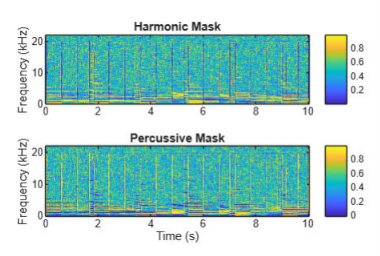
\includegraphics[width=1\linewidth]{Screenshot 2026-10-24 164600.png}
\caption{Harmonic and percussive soft masks for the real excerpt.}
\label{fig:masks}
\end{figure}

The waveforms in Fig.~\ref{fig:wave} are consistent with these observations. The harmonic waveform closely follows the original, with a similar amplitude range. The percussive waveform has a much smaller amplitude, with short bursts at the attack times and low activity in between.

\begin{figure}[t]
\centering
\includegraphics[width=1\linewidth]{waveforms.png}
\caption{Time-domain waveforms of the original signal and the harmonic and percussive components.}
\label{fig:wave}
\end{figure}

\subsection{Effect of Mask Type and Filter Length on the Real Excerpt}
Table~\ref{tab:real} compares energy shares and reconstruction error for different configurations on the real excerpt. With soft masks, increasing $L$ from 9 to 17 to 31 raises the harmonic share from 81.9\% to 89.2\% to 94.8\% and lowers the percussive share from 2.7\% to 1.5\% to 0.8\%. Binary masks at $L=17$ give 96.5\% and 1.3\%. Their shares sum to 97.8\%, closer to 100\% than the soft-mask total of 90.7\%, which is consistent with binary masks assigning each time-frequency point to a single component so that the two outputs overlap less. The reconstruction error is at the level of numerical precision (below $10^{-15}$) in every configuration, so the choice of mask and filter length does not affect perfect reconstruction. The percussive share stays at or below 2.7\% throughout, which confirms that the excerpt is dominated by tonal content.

Energy share is not a measure of separation quality, and no reference stems exist for this excerpt. Table~\ref{tab:real} therefore shows how the energy split moves with the settings, but not which setting separates the excerpt best. Whether longer filters also separate real music better, as they did on the synthetic benchmark, cannot be determined without references.

\begin{table}[t]
\centering
\caption{Energy share and reconstruction error on the real excerpt ($N=1024$, $H=256$). }
\label{tab:real}
\begin{tabular}{lccc}
\toprule
Configuration & $E_H/E_x$ (\%) & $E_P/E_x$ (\%) & Recon.\ error\\
\midrule
Soft, $L=17$ & 89.2 & 1.5 & $8.01\times10^{-17}$\\
Binary, $L=17$ & 96.5 & 1.3 & $3.80\times10^{-32}$\\
Soft, $L=9$ & 81.9 & 2.7 & $7.46\times10^{-17}$\\
Soft, $L=31$ & 94.8 & 0.8 & $8.22\times10^{-17}$\\
\bottomrule
\end{tabular}
\end{table}

\subsection{Synthetic Benchmark}
Table~\ref{tab:sdr} reports the SDR of each component on the synthetic benchmark, where the references are known. The first row is the baseline in which the unseparated mixture is used as the estimate of each component. Because the harmonic part carries about 20 times the energy of the percussive part, this baseline is $+13.1$~dB for the harmonic reference and $-13.1$~dB for the percussive reference.

\emph{Mask type.} With the default settings, binary masks reach 21.24~dB for the harmonic component and 8.10~dB for the percussive component, against 15.09~dB and 1.94~dB for soft masks, a difference of about 6~dB in both components. Relative to the baseline, binary masks improve the harmonic SDR by 8.1~dB and the percussive SDR by 21.2~dB, and soft masks by 1.9~dB and 15.1~dB.

\emph{Filter length.} SDR increases monotonically with $L$ for both components, from 8.08~dB to 20.89~dB (harmonic) and from $-5.07$~dB to 7.74~dB (percussive). For $L=5$ and $L=9$ the harmonic SDR is below the mixture baseline of 13.14~dB, so short filters degrade the harmonic estimate, although the percussive estimate still improves on its baseline. The longest tested filter is the best, so the optimum lies beyond the tested range.

\emph{Window length.} SDR also increases with $N$, from 11.35~dB to 21.11~dB (harmonic) and from $-1.79$~dB to 7.97~dB (percussive). Because $L$ is fixed in bins and the hop is $N/4$, changing $N$ also changes the extent of the median filters. At 22.05~kHz the time median spans roughly 0.1~s at $N=512$ and 0.4~s at $N=2048$, and the frequency median spans roughly 730~Hz and 180~Hz respectively. The effects of window length and filter extent are therefore not separated in this experiment.

\emph{Noise.} With added white noise, the harmonic SDR falls from 15.09~dB to 14.64, 12.02, and 4.89~dB at 20, 10, and 0~dB SNR, and the percussive SDR falls from 1.94~dB to 1.47, $-1.20$, and $-8.31$~dB. The loss is below 0.5~dB at 20~dB SNR and large at 0~dB. Since the noise counts as distortion and the SDR of the noisy mixture was not computed, these figures show how quickly the score drops, not how much separation gain remains.

\begin{table}[t]
\centering
\caption{SDR on the synthetic benchmark ($N=1024$, $H=256$, $L=17$, soft mask unless stated; $H=N/4$ in the window sweep).}
\label{tab:sdr}
\footnotesize
\begin{tabular}{lcc}
\toprule
Setting & SDR$_H$ (dB) & SDR$_P$ (dB)\\
\midrule
Mixture used as estimate & 13.14 & $-13.14$\\
\midrule
Binary mask & 21.24 & 8.10\\
Soft mask & 15.09 & 1.94\\
\midrule
$L=5$ & 8.08 & $-5.07$\\
$L=9$ & 8.94 & $-4.20$\\
$L=17$ & 15.09 & 1.94\\
$L=31$ & 18.51 & 5.37\\
$L=51$ & 20.89 & 7.74\\
\midrule
$N=512$ & 11.35 & $-1.79$\\
$N=1024$ & 15.09 & 1.94\\
$N=2048$ & 21.11 & 7.97\\
\midrule
SNR $=\infty$ & 15.09 & 1.94\\
SNR $=20$~dB & 14.64 & 1.47\\
SNR $=10$~dB & 12.02 & $-1.20$\\
SNR $=0$~dB & 4.89 & $-8.31$\\
\bottomrule
\end{tabular}
\end{table}

\section{Discussion}
The real-excerpt results show that median-filter HPSS separates the two classes in the way the spectrogram geometry predicts: tonal ridges stay in the harmonic output and broadband onsets move to the percussive output, and the soft masks guarantee that nothing is lost, as the near-zero reconstruction error confirms. The low percussive energy share should be read as a property of the excerpt, because energy share does not measure separation quality. A component can hold little energy and still be separated well.

The filter length controls a trade-off. A longer median along time suppresses transients more completely but also blurs genuine note changes, and a longer median along frequency removes tonal peaks more completely but also smears sharp onsets \cite{fitzgerald2010}. The benchmark shows only one side of this trade-off. SDR kept rising up to $L=51$, probably because each synthetic chord is stationary for 2.5~s, so a long time median costs little. Real music with faster note changes would be expected to have an optimum at shorter lengths, but this was not tested. The same caution applies to the window length, where $N=2048$ was best and the result is confounded with filter extent, as noted above.

Binary masks scored about 6~dB higher than soft masks. This is consistent with soft masks sharing every time-frequency point between the two outputs, so some energy of each class leaks into the other component. SDR does not capture audible artifacts, however, and binary masks can introduce artifacts that this measure does not penalize. No listening tests were conducted. The default configuration used for the real excerpt (soft masks, $L=17$, $N=1024$) is also not the best configuration on the benchmark.

The soft masks also remain near 0.5 in low-energy regions, so background noise is shared by both outputs rather than assigned to one. This is visible in Fig.~\ref{fig:masks}.

\section{Limitations and Future Work}
First, the real evaluation uses a single 10~s excerpt without reference stems, so it relies on visual inspection and energy measures, and the findings cannot be generalized to other music. Second, the synthetic benchmark is much simpler than real recordings: the tonal part has no vibrato or glides, and the drum-like part has no pitched or sustained percussion, both of which are known to cause leakage. Third, the SDR used here is the simple form and not the full BSS Eval measure \cite{vincent2006}. Fourth, the median-filter lengths are specified in bins, so the same length corresponds to different durations and bandwidths when the window length changes. Fifth, the sweeps over $L$ and $N$ did not reach an optimum, the noise experiment has no noisy-mixture baseline, and the best settings were not combined in a single run. Sixth, the study does not compare against other HPSS methods or learned separation models.

Future work includes evaluation on a standard dataset with reference stems, a third residual component \cite{driedger2014}, multi-resolution STFT analysis, iterative median filtering, and specifying the filter lengths in milliseconds and hertz.

\section{Conclusion}
This paper implemented and studied harmonic-percussive source separation using the STFT and median filtering in MATLAB. On a 10~s music excerpt, the harmonic output preserved the sustained tonal ridges and the percussive output isolated the broadband onsets, and the two components reconstructed the original signal with negligible error. A synthetic benchmark with known references was used to quantify the effect of mask type, filter length, window length, and noise. Relative to using the mixture as the estimate, the default soft-mask method raised the percussive SDR from $-13.1$~dB to 1.9~dB, binary masks reached 8.1~dB, and SDR increased with filter length and window length up to the largest values tested ($L=51$, $N=2048$). The central conclusion is that median-filter HPSS is a simple and effective baseline whose behavior depends strongly on the filter and window settings, while evaluation on measured data with reference stems is needed to establish how well these findings carry over to real recordings.

\begin{thebibliography}{00}
\bibitem{muller2015} M. M\"uller, \emph{Fundamentals of Music Processing}. Cham, Switzerland: Springer, 2015.
\bibitem{uhle2003} C. Uhle, C. Dittmar, and T. Sporer, ``Extraction of drum tracks from polyphonic music using independent subspace analysis,'' in \emph{Proc. 4th Int. Symp. Independent Component Analysis and Blind Signal Separation (ICA)}, Nara, Japan, 2003.
\bibitem{ono2008} N. Ono, K. Miyamoto, J. Le Roux, H. Kameoka, and S. Sagayama, ``Separation of a monaural audio signal into harmonic/percussive components by complementary diffusion on spectrogram,'' in \emph{Proc. EUSIPCO}, Lausanne, Switzerland, 2008.
\bibitem{fitzgerald2010} D. Fitzgerald, ``Harmonic/percussive separation using median filtering,'' in \emph{Proc. 13th Int. Conf. Digital Audio Effects (DAFx)}, Graz, Austria, 2010.
\bibitem{tachibana2014} H. Tachibana, N. Ono, H. Kameoka, and S. Sagayama, ``Harmonic/percussive sound separation based on anisotropic smoothness of spectrograms,'' \emph{IEEE/ACM Trans. Audio, Speech, Lang. Process.}, vol. 22, no. 12, pp. 2059--2073, Dec. 2014.
\bibitem{driedger2014} J. Driedger, M. M\"uller, and S. Disch, ``Extending harmonic-percussive separation of audio signals,'' in \emph{Proc. Int. Soc. Music Information Retrieval Conf. (ISMIR)}, Taipei, Taiwan, 2014.
\bibitem{allen1977} J. B. Allen, ``Short term spectral analysis, synthesis, and modification by discrete Fourier transform,'' \emph{IEEE Trans. Acoust., Speech, Signal Process.}, vol. 25, no. 3, pp. 235--238, Jun. 1977.
\bibitem{griffin1984} D. W. Griffin and J. S. Lim, ``Signal estimation from modified short-time Fourier transform,'' \emph{IEEE Trans. Acoust., Speech, Signal Process.}, vol. 32, no. 2, pp. 236--243, Apr. 1984.
\bibitem{oppenheim} A. V. Oppenheim and R. W. Schafer, \emph{Discrete-Time Signal Processing}, 3rd ed. Upper Saddle River, NJ, USA: Pearson, 2010.
\bibitem{vincent2006} E. Vincent, R. Gribonval, and C. F\'evotte, ``Performance measurement in blind audio source separation,'' \emph{IEEE Trans. Audio, Speech, Lang. Process.}, vol. 14, no. 4, pp. 1462--1469, Jul. 2006.
\end{thebibliography}

\end{document}
